\documentclass[../thesis.tex]{subfiles}
\begin{document}

\chapter{Preliminaries}
\label{ch:prelim}
As mentioned above, the existing system simulates and analyzes a tissue-level model of segmentation clock network. In this stage, I will focus on improving runtime of the existing CPU only system by introducing GPU acceleration to the system. 
\section{Methodology: }
\subsection{CUDA Platform}
In this study, I chose CUDA by NVIDIA as the platform for GPU computing. As a minimal extension of C and C++, CUDA works well with the existing system and it has been applied to create scalable parallel programs in similar disciplines such as computational chemistry \cite{nickolls2008scalable}. There are three key abstractions in the CUDA platform: a hierarchy of thread groups, shared memories, and barrier synchronization. Together, those three abstractions create a parallel structure to C/C++ code. This structure allows coarse-grained parallelism on the high level and more fine-grained parallelism on lower levels. It is a perfect candidate for executing simulations in a biological regulatory network since the structure within the CUDA platform corresponds well to a large computational model. In particular, CUDA platform is organized as grids of blocks where each block contains a set of parallel threads, the lowest level of parallelism in the system. The set of threads in a block cooperates well with barrier synchronization and shared access to a memory space private to the block.  Each thread is analogous to a cell inside one single simulation since cells are simulated in parallel to each other and the set of all cells in a simulation are connected and need to share common memory. On a higher level, parameter estimation contains a set of simulations that are not related to each other and can execute in parallel, exactly corresponding to a gird of independent block that can be executed independently. Overall, CUDA platform and its design correspond with a biological system from low level to high level simulations.
\subsection{Initial Attempt}
Conversion of the original system to GPU started with simulation of all six mutants (of a parameter set) in parallel for one parameter set. Under this scheme, the system is broken into three major parts: All inputting parameters, creating new data structures, and copying original code to new copies are executed in the original order for each of the mutants. A \textit{for loop} is added to iterate and setup all six mutants before the system moves to the next phase. Next, the system transfers all the data necessary for simulation (particularly data needed by protein synthesis, dimer synthesis and mRNA synthesis) to GPU and the system starts one block on GPU for simulating each of the six mutants. During simulation of a single time step, the system transfers relatively small portions of data between CPU and GPU for the purposes of updating rates and storing intermediate concentration levels. This part of the program is executed in parallel on GPU. After all simulations of this time step have completed on GPU, the system then copy all data back to CPU. The same process repeats for all time steps, and once simulation of all time steps is complete, the system starts to perform feature extraction and testing for all mutants. Similar to the first phase, all processes in the last phase are executed in the same order as they were originally, except there is a new \textit{for loop} over six mutants.\\
\\
 	The major difficulty in this part of the project is minimizing data transfer between CPU and GPU. Since rates of reaction, concentration level of mRNAs and proteins all need to be updated and stored at each occurrence. Large amounts of data transfer may likely be inefficient and dismiss the benefit of incorporating GPU computing into the system. This is because GPU has to constantly wait until all data transfer is completed and thus its computation power is far from being fully utilized. Therefore, I applied several methods to prevent data transfer to be the bottleneck of the heterogeneous computing system. 
	
\subsection{Improved Version}
To achieve an improvement of data transfer, I first integrated memory transfer of all six mutants together because transfer bundling is faster than transferring the same amount of data over separate occurrences. Next, I moved data transfer outside of the \textit{for loop} over all time steps. Now, the system transfers all data onto GPU in the beginning of the large \textit{for loop} over all time steps. Now data transfer of the entire data set only occurs twice for all time steps, instead of twice for each time step. In addition, I divided the transfer functions into two separate functions. One function will allocate a CPU array on the GPU and the other function will transfer the data and swap pointers to the array on GPU and CPU. I then added another function that will only swap pointers to the array. Through those separated functions, the system only needs to allocate the array once and can access the array repeatedly later using the pointer and swapping functions. The allocation process is now omitted during each data transfer, and the system only needs to overwrite the data at the given location; thus, each data transfer can be accelerated.\\
\\
	Less communication between GPU and CPU will obviously reduce unnecessary overheads and improve runtime of each individual simulation. However, less data transfer between CPU and GPU will require more data to stay on GPU throughout each simulation and will directly affect memory requirement of each process. When I was trying to simulate multiple parameter sets at the same time, simulation of multiple parameter sets lead to another challenge -- reducing the memory requirement of the simulation on GPU. Limited by the structure of the current system, the system keeps a copy on CPU for every copy of data structure existing on GPU. With large requirement on memory for each simulation, only a small number of simulations can fit on the GPU card simultaneously, and thus, utilization of GPU card does not reach its full capacity. \\
	\\
There are two viable ways to reduce the memory requirement of the system on GPU. The first way to reduce memory requirement is to increment time step and thus indirectly decrease the size of $baby\_cl$. If the time step is increased to 0.02, then size of $baby\_cl$ can reduce by half. Similarly, if time step if four time larger, then size of $baby\_cl$ can be reduced to a quarter of the original size. This change can be easily achieved; however, time step granularity (size of a time step) is directly determined by the accuracy requirements of the system. In other words, increasing step granularity may lead to less accurate simulation results. The second solution involves directly reducing the size of main data structure that will be copied to GPU. Currently, the number of time steps that every $baby\_cl$ keeps is the same and is equal to the maximum delay. However, most reactions require data from a small number of past time steps. If $baby\_cl$ for each of the reactions can be tailored according to the delay size of that reaction, memory requirement on GPU can reduced by a factor of six or ten in the worst and best case scenarios, respectively. Redesigning the data structure and changing time step sizes for differential equations require various changes over the entire program, and thus, they were not implemented in this preliminary stage. Instead, they will be addressed and incorporated during the later stages of the project.
\section{Results}
At the end of the preliminary stage, I obtained the following results: runtime of the system simulating one parameter set sequentially and in parallel are 6:15 and 4:18, respectively. Runtime for simulating two parameter sets in parallel is 7:26, which is roughly 3:43 per parameter set (Figure \ref{fig:result1}). 
\begin{figure}[h]
\centering
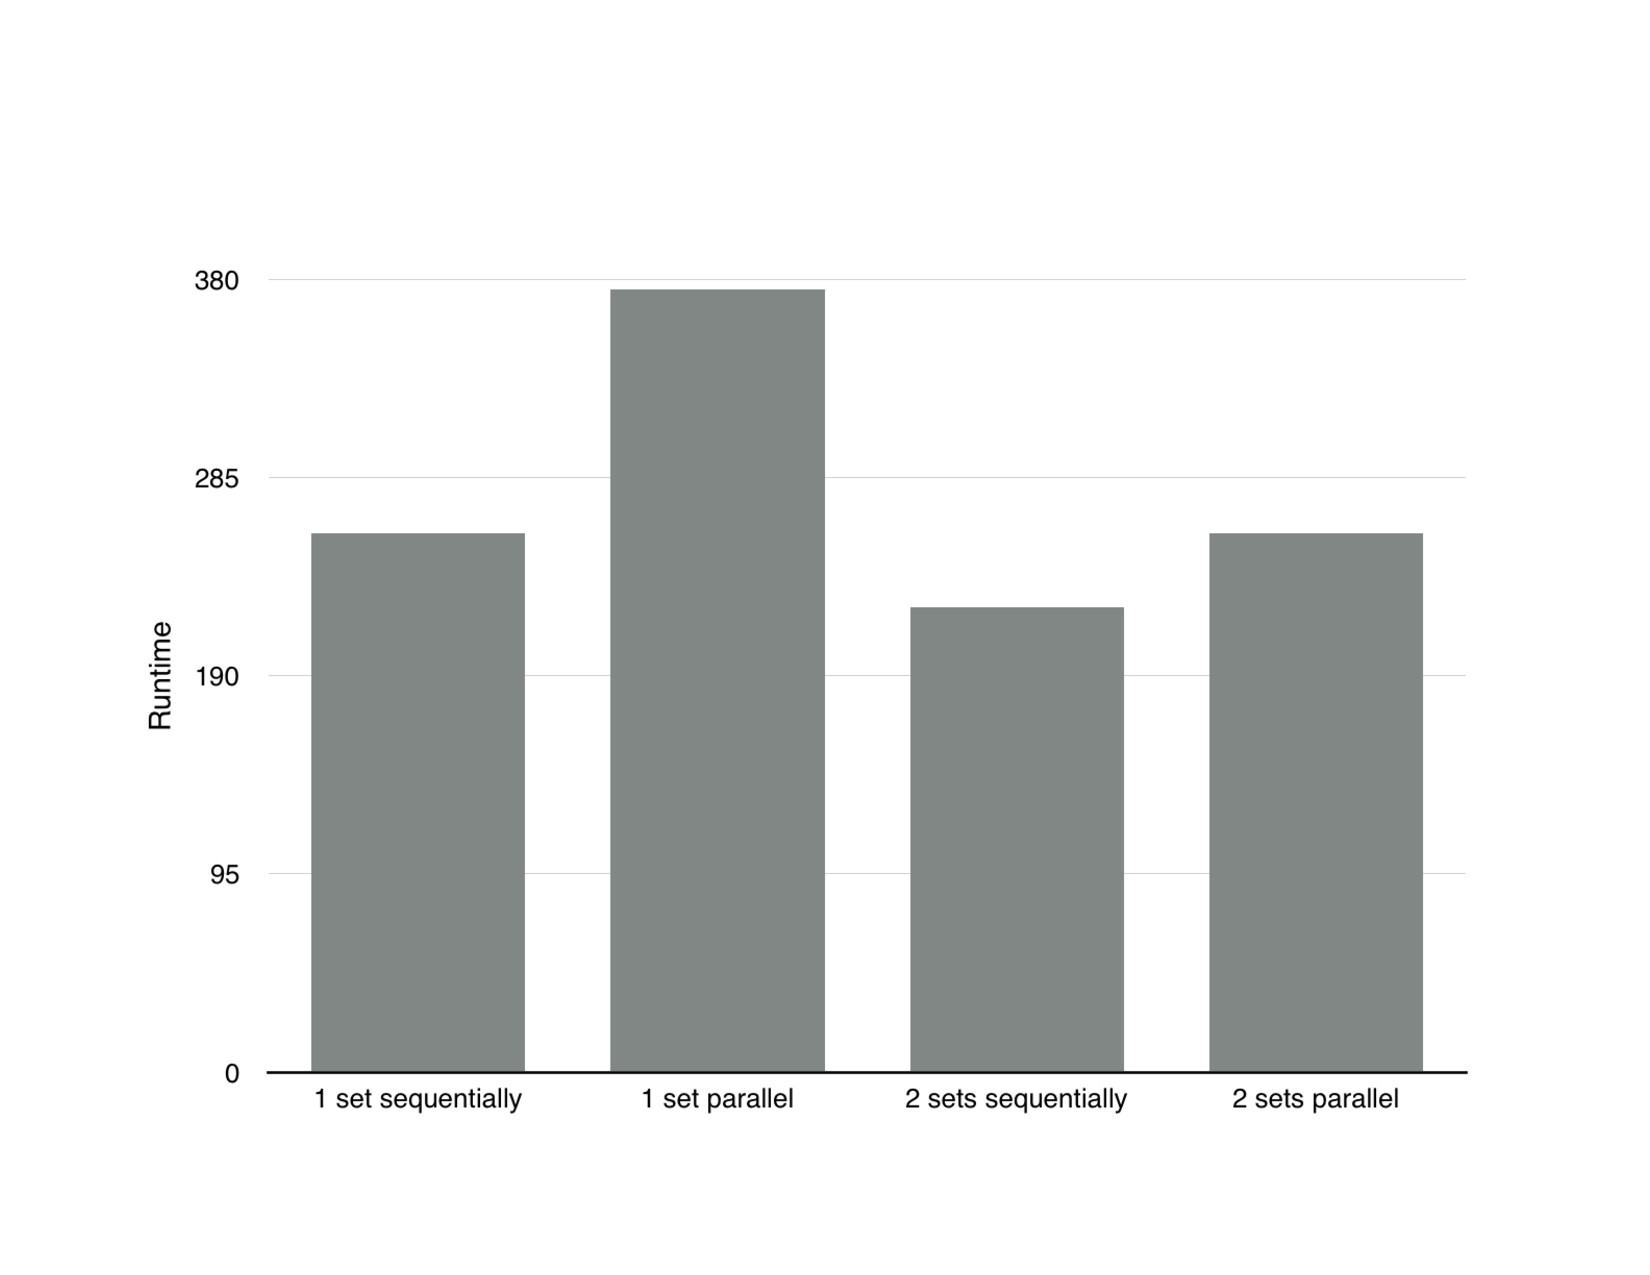
\includegraphics[width=0.9\textwidth]{ini_result1}
\caption{Runtime Per Parameter Set for Sequential and Parallel Simulations}
\label{fig:result1}
\end{figure}
Although the simulation runtime for one parameter set increases on GPU, improvements can be seen when multiple parameter sets are simulated. Instead of a linear increase in total runtime, GPU accelerated system has a much smaller increase since simulation, the most time-consuming part, is now executed in parallel with other sets and thus, does not incur additional runtime increase. Only feature extraction and analysis result in a light increase in average runtime. This pattern runtime increase continues to hold true with larger number of parameter sets, but before significant increase, the memory on GPU exhausts due to the reasons mentioned above.\\
\\
Overall, this is a successful experiment and reveals several factors in the current system that may affect the runtime. Data structures are larger than they need to be and thus inefficient. Due to this reason, number of parameter sets to be simulated on GPU at the same time is strictly limited. Furthermore, there are two copies of some data structures in the system, which increases memory requirement. Problems identified in this stage provide insights about limiting factors of current system and will be addressed during development of the new system. 
\end{document}

